
\chapter{Renderización de Geometrías Porosas}
\section{Introducción}
Debido a las limitaciones existentes actualmente en el renderizado realista de geometrías porosas en tiempos interactivos, nos proponemos en este capítulo estudiar la utilización de renderizado directo de volúmenes (Direct Volume Rendering, \acrshort{DVR} \cite{Kratz2006}), aplicado a un campo escalar representando la geometría del material. 
Los resultados obtenidos son realistas y se renderizan en tiempo real. La misma evita el uso de estructuras intermedias, simplificando el desarrollo y reduciendo los costos computacionales.

El renderizado foto-realista de materiales con una estructura interna compleja presenta grandes retos en computación gráfica.
En particular, los materiales porosos son translúcidos y complejos, presentando detalles dispares en distintas escalas, todos igualmente necesarios de ser tenidos en cuenta para lograr una correcta visualización.
El renderizado realista de estos materiales debe simular correctamente diversos fenómenos como translucencia, auto-sombreado, auto-oclusión, reflectancia, y absorción, entre otros.

Las técnicas del estado del arte en renderizado de materiales porosos tratan el material como una superficie, capturando sus propiedades por medio de un complejo procedimiento en el cual la luz reflejada por el material se fotografía desde distintos ángulos.
Posteriormente la información se procesa y reconstruye para formar un modelo del material.
Si bien esta solución captura adecuadamente los fenómenos lumínicos previamente discutidos, también es cierto que la practicidad del método se encuentra severamente comprometida, presentando un elevado costo computacional, un procedimiento de captura muy limitado y la imposibilidad de obtener más de una apariencia con una única captura.

En un intento por superar estas limitaciones, proponemos utilizar la técnica de DVR, la cual implementamos en \acrshort{GPU}, utilizando el lenguaje de shader GLSL (ver Apéndice A).
La técnica permite renderizar los campos escalares computados en el capítulo anterior sin utilizar estructuras intermedias.
Las imágenes obtenidas son promisorias, y se computan en tiempo real gracias al poder de las placas gráficas actuales.

\section{Trabajo Previo}
El tópico de renderizado foto-realista de materiales, y su modelado, atrajo un interés creciente en la literatura científica.
La mayoría de los esfuerzos están focalizados en materiales complejos de frecuente aparición como el agua \cite{Schechter2012}, la piel humana \cite{Donner2006}, metales, plásticos \cite{Kurt2010}, etc.
La comunidad de investigadores, sin embargo, ha tenido grandes dificultades para simular adecuadamente la apariencia de otros materiales, como en el caso de materiales cocidos ({\em e.g.}, pizza, galletitas).
Debido a su compleja geometría y fenómenos lumínicos involucrados, esto continúa siendo un problema abierto \cite{Voglsam2013}.

En los últimos años, el costo computacional de renderizar modelos físicos de estos materiales resultaba prohibitivo si el tiempo real era un requerimiento.
De todas formas, el crecimiento notable en poder de cómputo debido al diseño masivamente paralelo de las placas gráficas \cite{Yeo09,Harris06}, está permitiendo la simulación de fenómenos complejos de interacción de la energía radiante con materiales en tiempos de cómputo aceptables.

%Simular un modelo geométrico aceptable representa un reto adicional, como fue visto en el capítulo anterior.
%El pan y otras estructuras porosas son el resultado de mecanismos complejos que involucran deformaciones físicas, transferencia de masa y calor durante la cocción, y distintas reacciones químicas.

Estudios recientes utilizan consideraciones fenomenológicas sobre materiales porosos, pero la geometría resulta invariable (es decir, no procedimental) \cite{VanDyck2014}: una geometría fija no permite obtener diferentes tipos de pan fácilmente, ya que requiere un procedimiento de captura para cada uno de ellos.
Adicionalmente, las distribuciones de burbujas no pueden ser controladas.

La presencia de mesoestructuras (burbujas con formas complejas) provocan una clasificación de los materiales porosos como {\em cuasi-homogéneos} \cite{Tong2005}. 
Por esta razón, modelar al material como una superficie no resulta adecuado.
Técnicas típicas como BRDFs, BSSRDFs \cite{Donner2009} y BTFs, no resultan satisfactorias.
Una publicación intenta resolver las limitaciones \cite{Tong2005}, pero las desventajas que acarrea (proceso de captura muy complejo, altos costos computacionales, invariabilidad geométrica), resultan en un proceso basado en fuerza bruta y muy poco práctico.

\section{Renderizado Directo de Volúmenes (DVR)}

La técnica de DVR genera imágenes bidimensionales computando la interacción de la luz con un medio semi-transparente, el cual se representa a través de un campo escalar discreto.
Este campo describe la densidad del medio en cada celda discretizada.
Para cada píxel en la imagen final, se computa un rayo desde la posición de la cámara en el espacio virtual, y la radiancia que alcanza la cámara desde esa dirección se computa aproximando la RTE en su forma integral, ec. (\ref{eq:rteintegral}).
Esta ecuación describe la modificación de radiancia a medida que el rayo atraviesa el medio no transparente.
En su forma completa, la RTE incorpora muchas propiedades ópticas y efectos.
Para aproximar el resultado de la RTE en tiempo real, este capítulo utiliza una versión simplificada de la ecuación que sólo toma en consideración algunos de los fenómenos ópticos que ocurren en la realidad.

Como fue explicado en el Capítulo $2$, existen tres fenómenos ópticos importantes que afectan la propagación de la luz a través de un medio en un punto dado del espacio: emisión, absorción, y dispersión.
La emisión se define como la generación de energía radiante en una dirección dada.
La absorción ocurre cuando una fracción o toda la energía radiante en el rayo de luz se topa con un objeto opaco transformándose en otras formas de energía.
Finalmente, la dispersión produce modificaciones de dirección en los fotones.
Aquellos eventos que provocan que los fotones modifiquen su dirección a otra distinta a la dirección del rayo, son llamados de dispersión saliente. Del mismo modo, los eventos que provocan que los fotones modifiquen su dirección por la del rayo actual se llaman dispersión entrante.

%
La contribución de la dispersión entrante en la radiancia se computa a partir de una única dirección, la cual corresponde a la principal fuente de luz de la escena.
Esto aproxima la energía radiativa que llega a un punto desde la fuente de luz, haciendo rebotar a las partículas en el medio hacia ese punto y luego viajando a lo largo de una dirección dada. 

La RTE puede reescribirse a partir de la ecuación (\ref{eq:rteintegral}), para ser utilizada en DVR como sigue,

\begin{equation} \label{eq:general_radiance}  
  L(p_n) = L_b + \int_{p_0}^{p_n} \frac{\partial L(t)}{\partial p} \, dt,
\end{equation}

\noindent donde $L_b$ es la radiancia de fondo, y $p_0$, $p_n$ son los puntos visibles más cercano y más lejano en la dirección del rayo, respectivamente, $L(t)$  es la radiancia en el punto $t$, y $\partial p$ es la distancia entre puntos consecutivos muestreados. 
Debido a que la entrada del algoritmo de DVR constituye un conjunto de datos discreto, la integral en $L(p_n)$ se aproxima por una suma.

La extinción constituye el descenso de radiancia en un rayo debido a absorción y dispersión saliente.
Podemos aproximar este efecto definiendo un coeficiente de absorción para el medio, $k_a$ y un coeficiente de dispersión saliente $k_s$. 
Si descartamos el efecto de dispersión saliente, la fórmula que describe la radiancia alcanzando un punto luego de atravesar un segmento de un rayo es:

\begin{equation} \label{eq:radiance_absorption}  
    L_b \ e^{- \textstyle  \int_{p_0}^{p_n} k_a(t) \, dt}.
\end{equation}

Introducimos el valor $\int_{p_i}^{p_j} k_a(t) \, dt$, el coeficiente de absorción, el cual referiremos como $\tau_{(p_i, p_j)}$. 
La transmitancia representa el concepto complementario a la extinción, describiendo la cantidad de luz que escapa a un medio en una dirección dada.
Por lo tanto, el valor de la transmitancia entre dos puntos $p_i$ y $p_j$ es:

\begin{equation} \label{eq:transmittance}  
  T(p_i,p_j) = e^{- \textstyle \tau_{(p_i, p_j)}}.
\end{equation}

Asumiendo un incremento en la radiancia en cada punto del rayo dentro del volumen, dada por la dispersión entrante y fenómenos de emisión ($\rho$), luego nuestra estimación inicial de radiancia resulta,

\begin{equation} \label{eq:ray_radiance}  
  L(p_n) = L_b \ e^{-\tau(p_0, p_n)} + \int_{p_0}^{p_n} \rho \ e^{-\tau(t,p_n)} \, dt.
\end{equation}

Esto significa que la radiancia a lo largo de los puntos $p_0$ y $p_n$ es la radiancia de fondo atenuada, más la emisión y la dispersión entrante atenuadas en cada punto del rayo.

El algoritmo de DVR muestrea la función de densidad del volumen a intervalos regulares, aproxima la transmitancia a lo largo de esos puntos y computa la cantidad de luz que llega a la cámara a lo largo de la dirección del rayo.
La computación reemplaza la suma integral por una suma discreta sobre el rayo intersectando el volumen,

\begin{equation} \label{eq:ray_radiance}  
  L(p_n) = L_b \ e^{-\tau(p_0, p_n)} + \sum_{p_0}^{p_n} \rho \ e^{-\tau(p_i,p_n)}.
\end{equation}

Es posible tener en cuenta otros efectos, aumentando la fidelidad de la imagen final, así como los costos computacionales de la técnica.
La base de nuestro algoritmo de renderizado utiliza un modelo simplificado que sólo tiene en cuenta transmitancia $T$, emisión constante y dispersión entrante $\rho$ (aproximada a través del cómputo de la radiancia desde cada punto hacia la luz), junto con ciertas consideraciones artísticas, para alcanzar tasas de refresco de tiempo real.
Describiremos el algoritmo de renderizado en detalle en una sección posterior.

\section{Implementación}

Se creó una aplicación demo\footnote{disponible en \emph{https://www.github.com/rbaravalle/Pysys}}  que usa el sistema de partículas descrito en secciones previas para renderizar panes en tiempo real, utilizando DVR.
La Fig.~\ref{fg:application} muestra la aplicación desarrollada, con un objeto poroso renderizado en tiempo real.
En la demo se produce una textura volumétrica, renderizando un cubo que corresponde a esta textura en la escena.
El material utilizado para renderizar el cubo consta de un shader de vértices muy simple, y un shader de fragmentos, el cual implementa el algoritmo de DVR.
Para cada fragmento, el shader computa un rayo con origen en la posición de la cámara y con la dirección del fragmento que debe ser coloreado.
El procedimiento muestrea la textura volumétrica a intervalos regulares sobre la intersección del rayo y el cubo.
Estos valores muestreados son luego utilizados como entrada de un algoritmo que implementa la Ec. (\ref{eq:ray_radiance}), computando el color del píxel resultante de la manera descrita en secciones previas.



\begin{figure}
\centerline{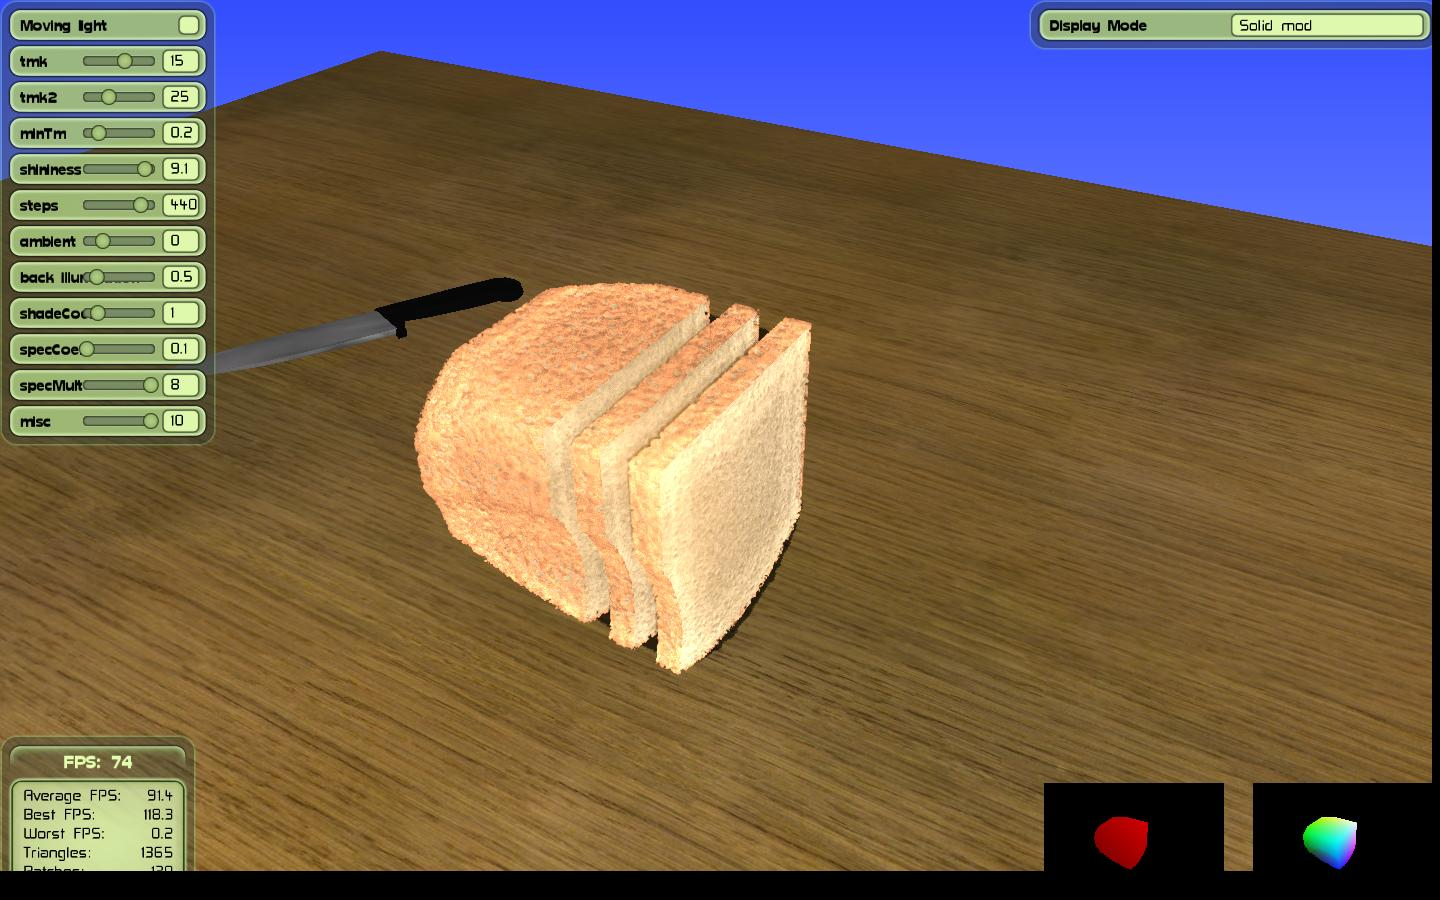
\includegraphics[width=11cm]{figures/application}}
\caption{Aplicación desarrollada mostrando una estructura porosa renderizada en tiempo real.}
\label{fg:application}
\end{figure}


La implementación acumula la transmitancia a lo largo del rayo y la contribución de radiancia en cada punto muestreado.
La computación termina si el valor de la transmitancia acumulada está por debajo de un umbral (lo cual significa que no escaparán más fotones en el rayo) o si el rayo sale del cubo.
La dispersión entrante ($\rho$), simplificada, se computa a través de un rayo secundario, para cada punto muestreado, en dirección a la fuente de luz.
Este rayo secundario se muestrea para determinar la cantidad de luz que llega al punto.
Esta técnica permite obtener sombras naturales dentro del volumen.
El píxel se sombrea utilizando la información de transmitancia del rayo primario y los secundarios en cada punto.
En este punto, diferentes consideraciones artísticas pueden ser aplicadas para obtener diferentes materiales con distintos aspectos.
Por ejemplo, podemos diferenciar miga de corteza asignando un coeficiente de extinción mayor y un color más oscuro a las regiones de corteza.
En nuestro caso, se aplica un color amarillo suave en ciertas regiones, otorgándoles una apariencia de miga.
Adicionalmente se puede agregar una sutil reflexión especular.
Para esto, se necesita computar la primera intersección entre el rayo y la geometría.
Gracias a esto se puede incrementar ligeramente el realismo final de la imagen.
El vector normal usado en este cálculo está dado por el gradiente de la textura volumétrica en ese punto.

La demo presentada provee al usuario la habilidad de modificar parámetros como el coeficiente de absorción, el umbral de transmitancia, los colores asignados y la visibilidad de los reflejos especulares.
Con la modificación de estos parámetros, el usuario puede producir imágenes que semejan distintos materiales porosos, como las esponjas, budines, panes o piedras.
La Fig. \ref{fg:fragmentshaderrte} muestra un esquema del shader de fragmentos implementado, donde se computa la Ec. (\ref{eq:ray_radiance}).

\begin{figure}[htb!]
\centerline{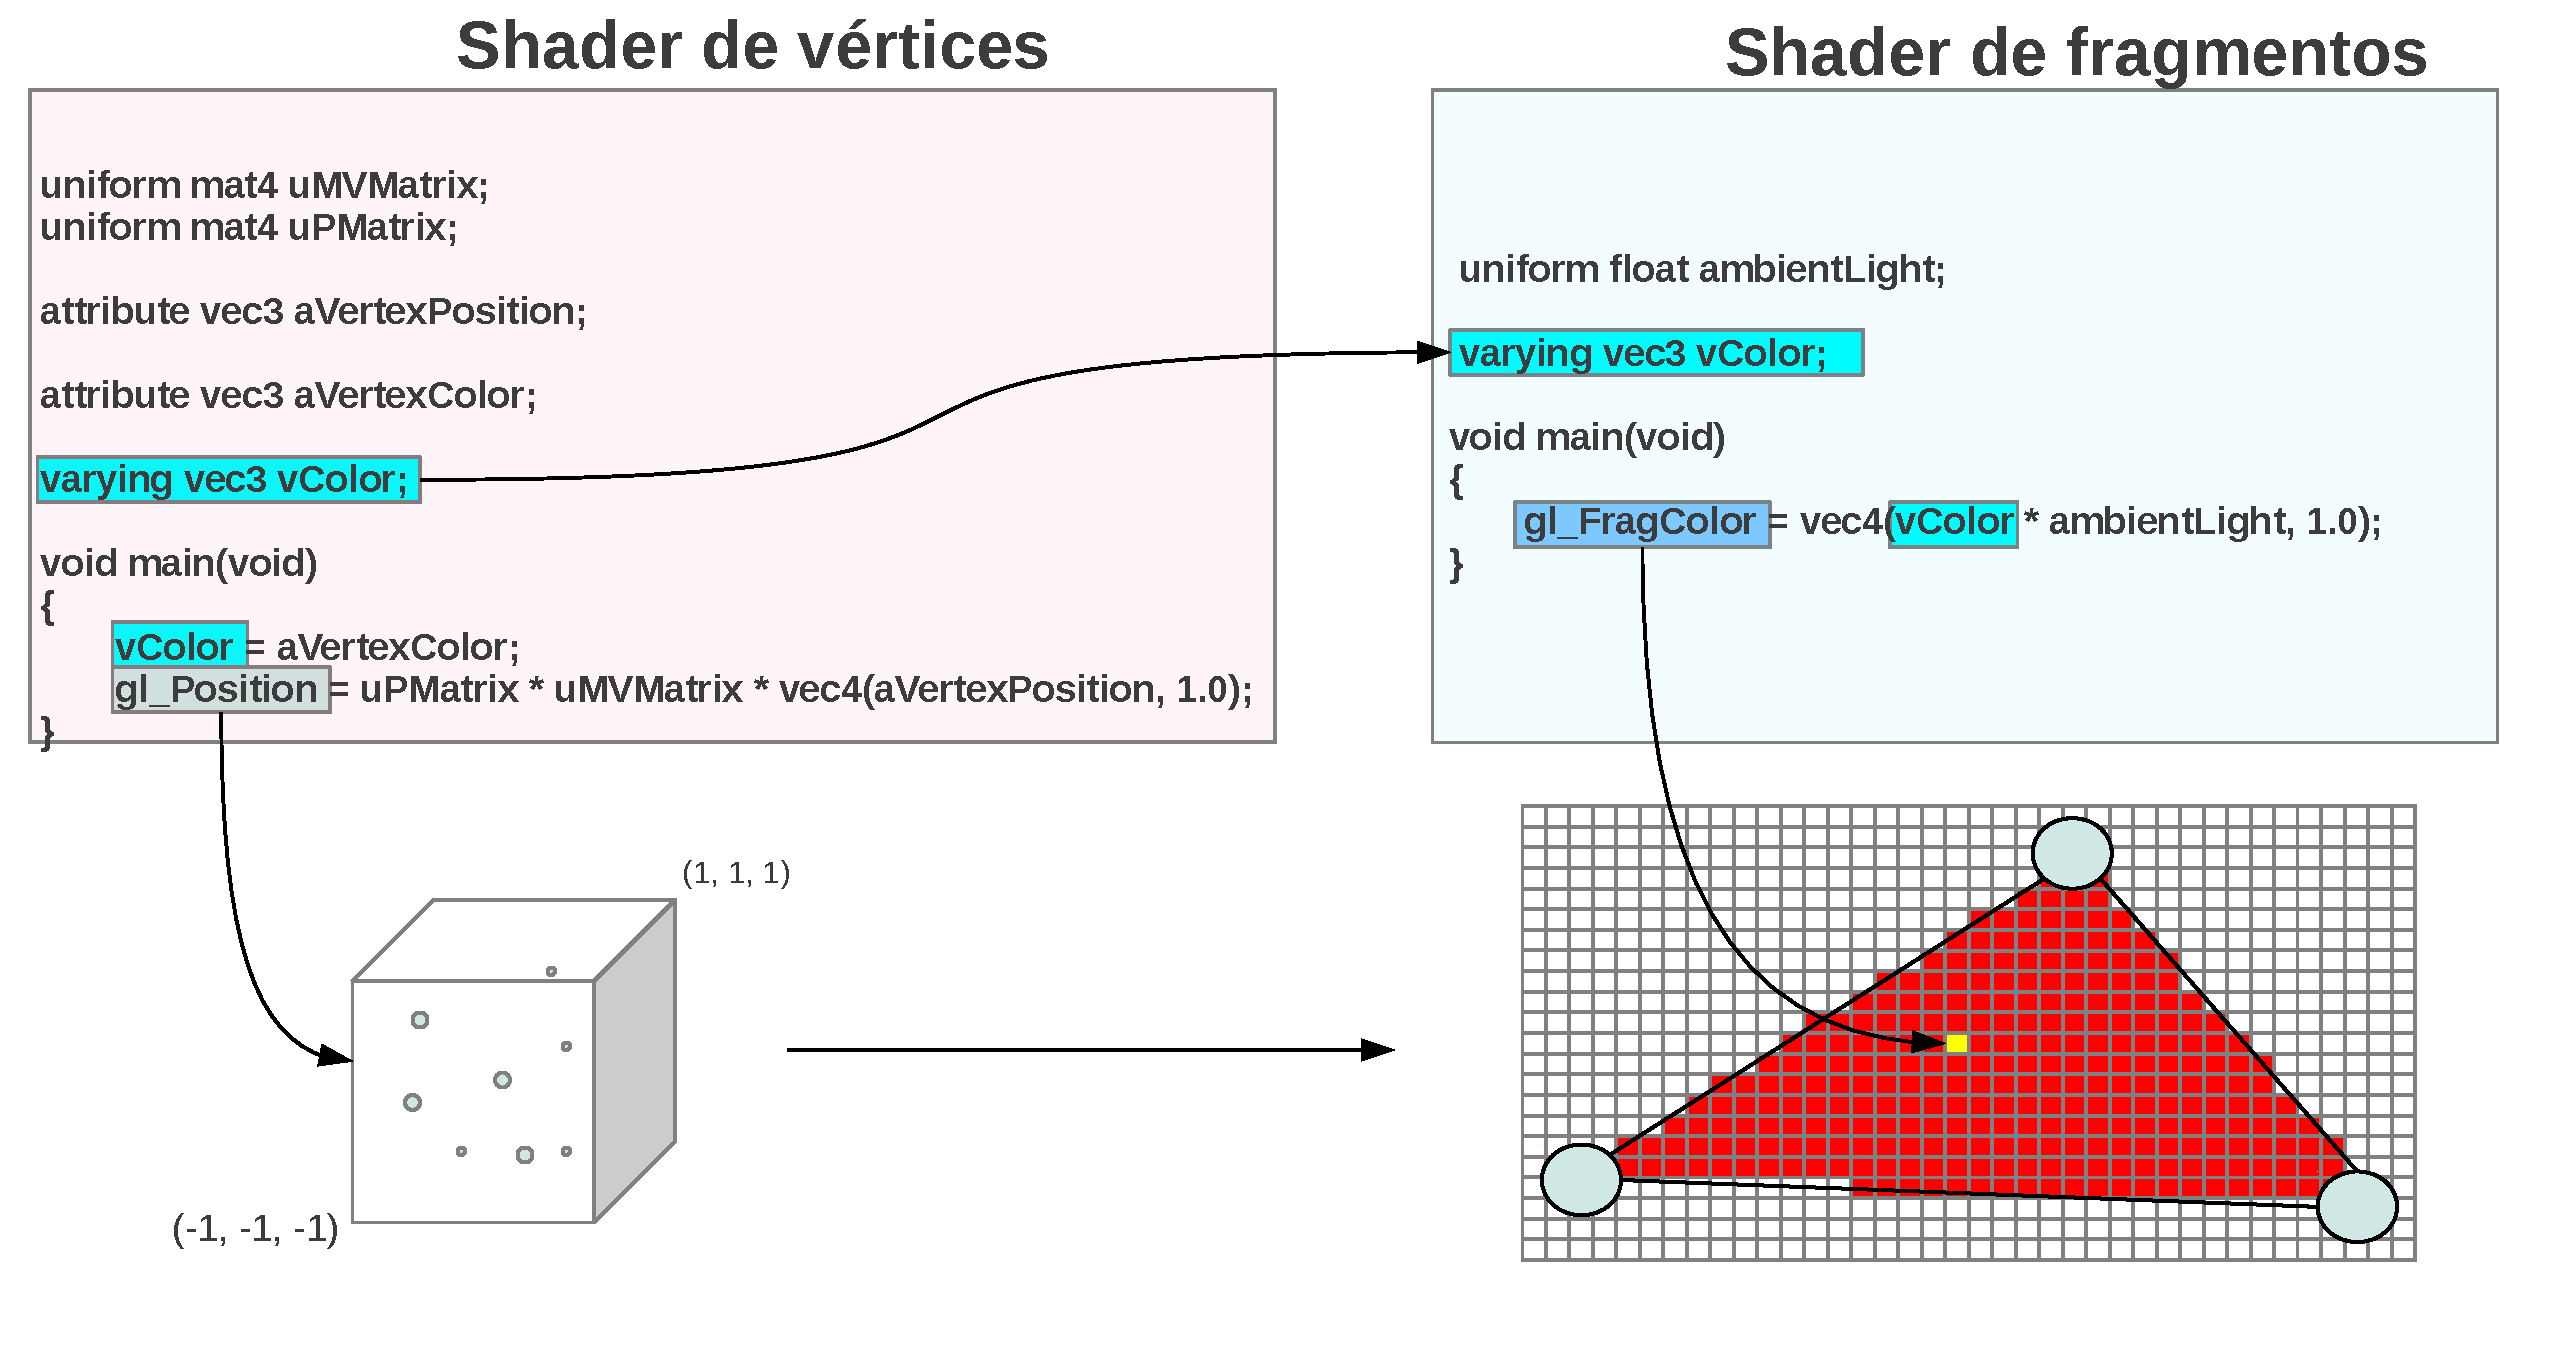
\includegraphics[width=9cm]{figures/fragmentshader}}
\caption[Cálculo de color en el shader de fragmentos]{Cálculo de color en el shader de fragmentos. Se implementa la suma en la ecuación (\ref{eq:ray_radiance}). La suma devuelve un color que luego se colorea por medio de un parámetro del usuario. Además, luego se computarán las normales, sombras y oclusión de ambiente.}
\label{fg:fragmentshaderrte}
\end{figure}


\subsection{Oclusión Ambiente}

La aproximación introducida a la RTE no tiene en cuenta fenómenos clave en la obtención de imágenes realistas, como la dispersión entrante y la dispersión saliente.
Sin embargo, un aspecto clave para resaltar la apariencia de la imagen final está basada en las contribuciones locales de radiancia debido a características microscópicas propias del material.
Hasta ahora, la dispersión entrante, simple, era aproximada por medio del cómputo de la radiancia entrante en el punto desde la fuente de luz.
Es posible lograr aproximaciones más precisas tomando en consideración además la dispersión entrante al punto desde el medio, por medio del agregado de la oclusión ambiente.
La literatura muestra que considerarla produce imágenes de mayor realismo \cite{Hernell2010}.

Debido a estas consideraciones proponemos computar la dispersión entrante, múltiple, calculando de manera offline un término de oclusión del ambiente para cada voxel en el campo escalar y almacenándolo como una textura volumétrica extra, la cual se suple al shader de fragmentos, permitiendo así mantener los tiempos computacionales en tasas razonables.
Para cada voxel en la textura volumétrica resultante de alguno de los métodos del capítulo anterior, el cómputo de dicho término define un radio $r$, almacenando el valor medio de los voxels vecinos dentro de una esfera que contiene ese radio.
Luego, este valor se utiliza para modular la contribución de cada paso del rayo.
Experimentalmente encontramos que variar el valor de $r$ produce resultados visualmente indistinguibles, por lo cual cualquier valor mayor que $0$ puede utilizarse para el cómputo.
La Fig.~\ref{fg:occlusion} muestra el realce que produce este concepto, resultando en un aspecto clave de nuestra implementación, a la hora de producir imágenes creíbles. 



\begin{figure}
\centerline{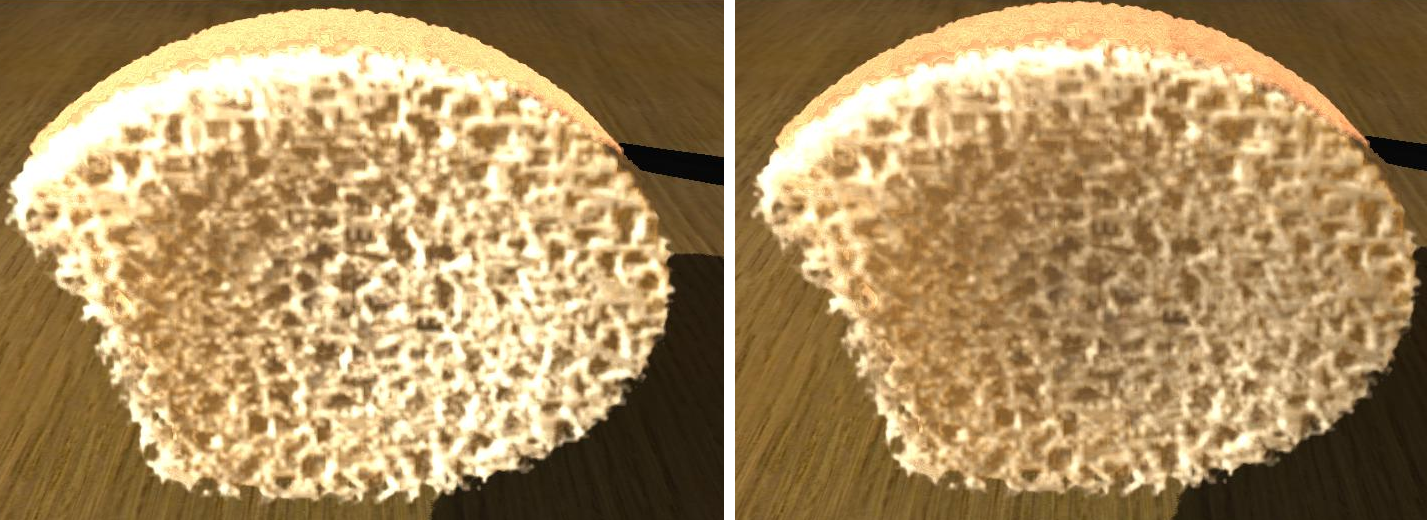
\includegraphics[width=10cm]{figures/occlusion}}
  \caption[Pan renderizado sin y con oclusión de ambiente]{Pan sin (izquierda) y con (derecha) oclusión de ambiente. La imagen final se realza notablemente, apreciándose una apariencia más natural.}
  \label{fg:occlusion}
\end{figure}
 
\subsection{Cómputo de las Normales}
El gradiente en el punto será utilizado para computar el vector normal en el modelo de iluminación.
Utilizamos un esquema {\em hacia adelante} en el cómputo de diferencias finitas del gradiente, el cual resulta de la diferencia normalizada, entre la posición {\em hacia adelante} y la posición actual del campo escalar,


\begin{equation}
\begin{aligned}
x &= tex(pos+\vec{i}) - tex(pos)\\
y &= tex(pos+\vec{j}) - tex(pos)\\
z &= tex(pos+\vec{k}) - tex(pos) \\
N &= normalizar([x,y,z])
\end{aligned}
\end{equation}

\noindent donde $\vec{i}$, $\vec{j}$ y $\vec{k}$ son los vectores unitarios que forman una base en $\mathbb{R}^{3}$.

La normal y el vector que representa la fuente de luz permiten determinar la contribución especular en el punto, aplicando un modelo de Phong con un exponente suave, y estableciendo un parámetro que permite al usuario especificar el impacto deseado para la componente especular.
Se han testeado otros modelos especulares más complejos, pero no se encontró diferencia apreciable en la apariencia final de la textura de pan.

\subsection{Cómputo de Sombras}
La técnica de DVR puede ser utilizada para computar sombras realistas, desde el objeto renderizado hacia la escena en la que se encuentra, por medio de mapas de sombras \cite{Williams1978}.
Durante la generación del mapa de sombras renderizamos nuevamente un cubo representando la geometría, pero esta vez los cómputos se realizan desde la posición de la fuente de luz.
El shader de fragmentos para ese cubo utiliza el mismo método de rayos explicado, pero solo computa la transmitancia en el rayo.
Si la transmitancia en ese rayo está por encima de un umbral al finalizar el cómputo (lo cual significa que cierta cantidad de fotones logran escapar al medio), luego el fragmento no corresponde a un oclusor, y su profundidad se establece a infinito.
Si durante el cómputo de la transmitancia, la misma cae por debajo del umbral, la profundidad del fragmento se establece en la profundidad alcanzada por el rayo en ese momento.

A partir de este cómputo obtenemos un mapa de sombras, el cual puede almacenarse como una textura.
Luego se computa DVR normalmente (desde el punto de vista del observador).
En este paso debe mapearse cada texel del mapa de sombras con una posición en el espacio, para determinar si el punto está en sombra o no.
Esta técnica se utiliza junto a un filtrado de porcentaje de cercanía, para generar sombras realistas en nuestra aplicación.
Casi todas las imágenes presentadas muestran el uso de esta técnica en nuestra aplicación.


\subsection{Corteza}
Se puede proveer al sistema con una función que indique si la posición es parte de una capa exterior o interior del material, u otras consideraciones (por ejemplo, si el color de la sección de una esponja debe ser amarillo o verde).
Una función puede definir una capa exterior cilíndrica asignando la etiqueta de ``capa interior'' a aquellas posiciones cercanas al eje del cilindro, y ``capa exterior'' a las restantes.

También se provee otra función que establece si la posición debe ser considerada parte del material o aire.
Esto permite definir de una manera intuitiva cortes en el volumen (ver Figs.~\ref{fg:breadsnooc} y \ref{fg:breads}).
Los métodos para definir la misma fueron explicados en el capítulo anterior por medio de la utilización de un mapa de distancias.


\section{Resultados}
Las imágenes obtenidas a partir del método descrito en la sección anterior fueron renderizadas en una computadora con una placa gráfica nVidia GTX 480 ($480$ cores), la cual normalmente se utiliza en hogares.
La CPU fue una Intel(R) Core(TM) i5-2300 CPU (cuatro procesadores).
La resolución de las imágenes es de $1440\times990$ pixels. 
Se obtuvieron diferentes imágenes que semejan materiales porosos y horneados.
Diferentes tipos de materiales pueden ser representados variando los parámetros de transmitancia y colores utilizados (ver Fig.~\ref{fg:breadsnooc}).
En esa imagen mostramos panes donde no se aplica oclusión de ambiente.
En la imagen central los patrones producidos por los sistemas de partículas descritos en el capítulo anterior son claramente visibles.
En ese caso, el tiempo de vida de las partículas difiere para cada una y de esa manera se obtienen burbujas de diferentes tamaños.

La Fig.~\ref{fg:breads} muestra panes renderizados en tiempo real con oclusión de ambiente agregada.
Puede observarse que los panes con este efecto muestran un grado de realismo superior.

\begin{figure*}[htb!]
  \centerline{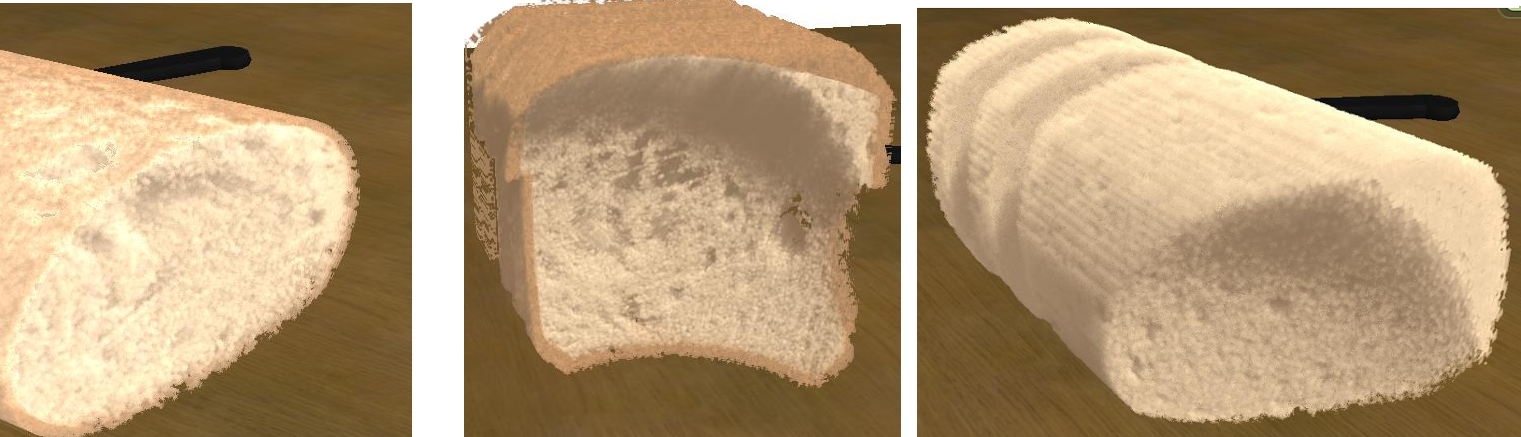
\includegraphics[width=12cm]{figures/fig5}}
  \caption[Imágenes de diferentes tipos de panes renderizados en tiempo real, sin oclusión de ambiente]{Imágenes de diferentes tipos de panes renderizados en tiempo real, sin oclusión de ambiente. La imagen de la derecha muestra un pan sin corteza}
  \label{fg:breadsnooc}
\end{figure*}


\begin{figure*}[htb!]
  \centerline{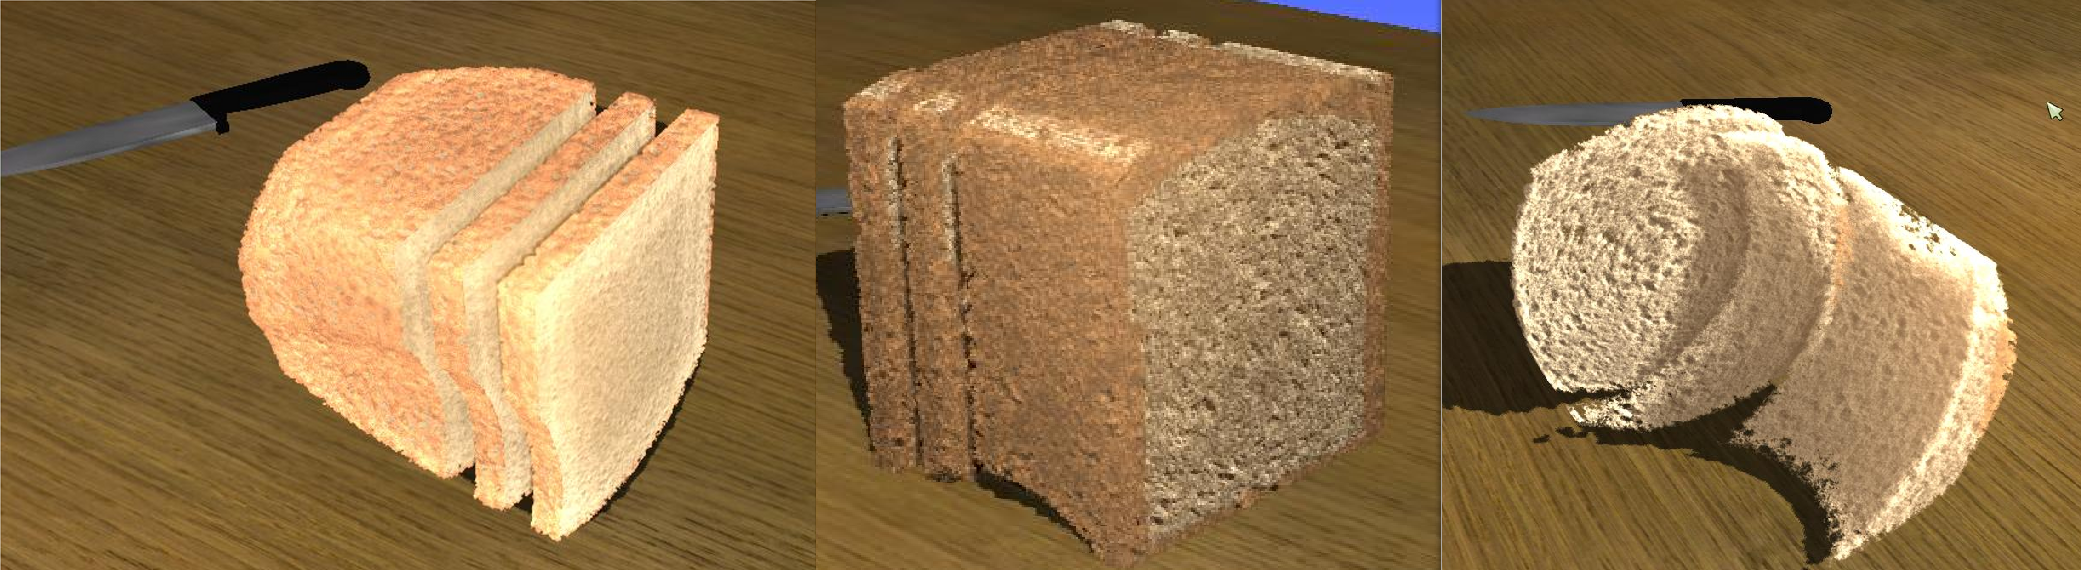
\includegraphics[width=12cm]{figures/breads}}
  \caption{Imágenes de diferentes tipos de panes renderizados en tiempo real, con oclusión de ambiente.}
  \label{fg:breads}
\end{figure*}


\begin{figure}
  \centerline{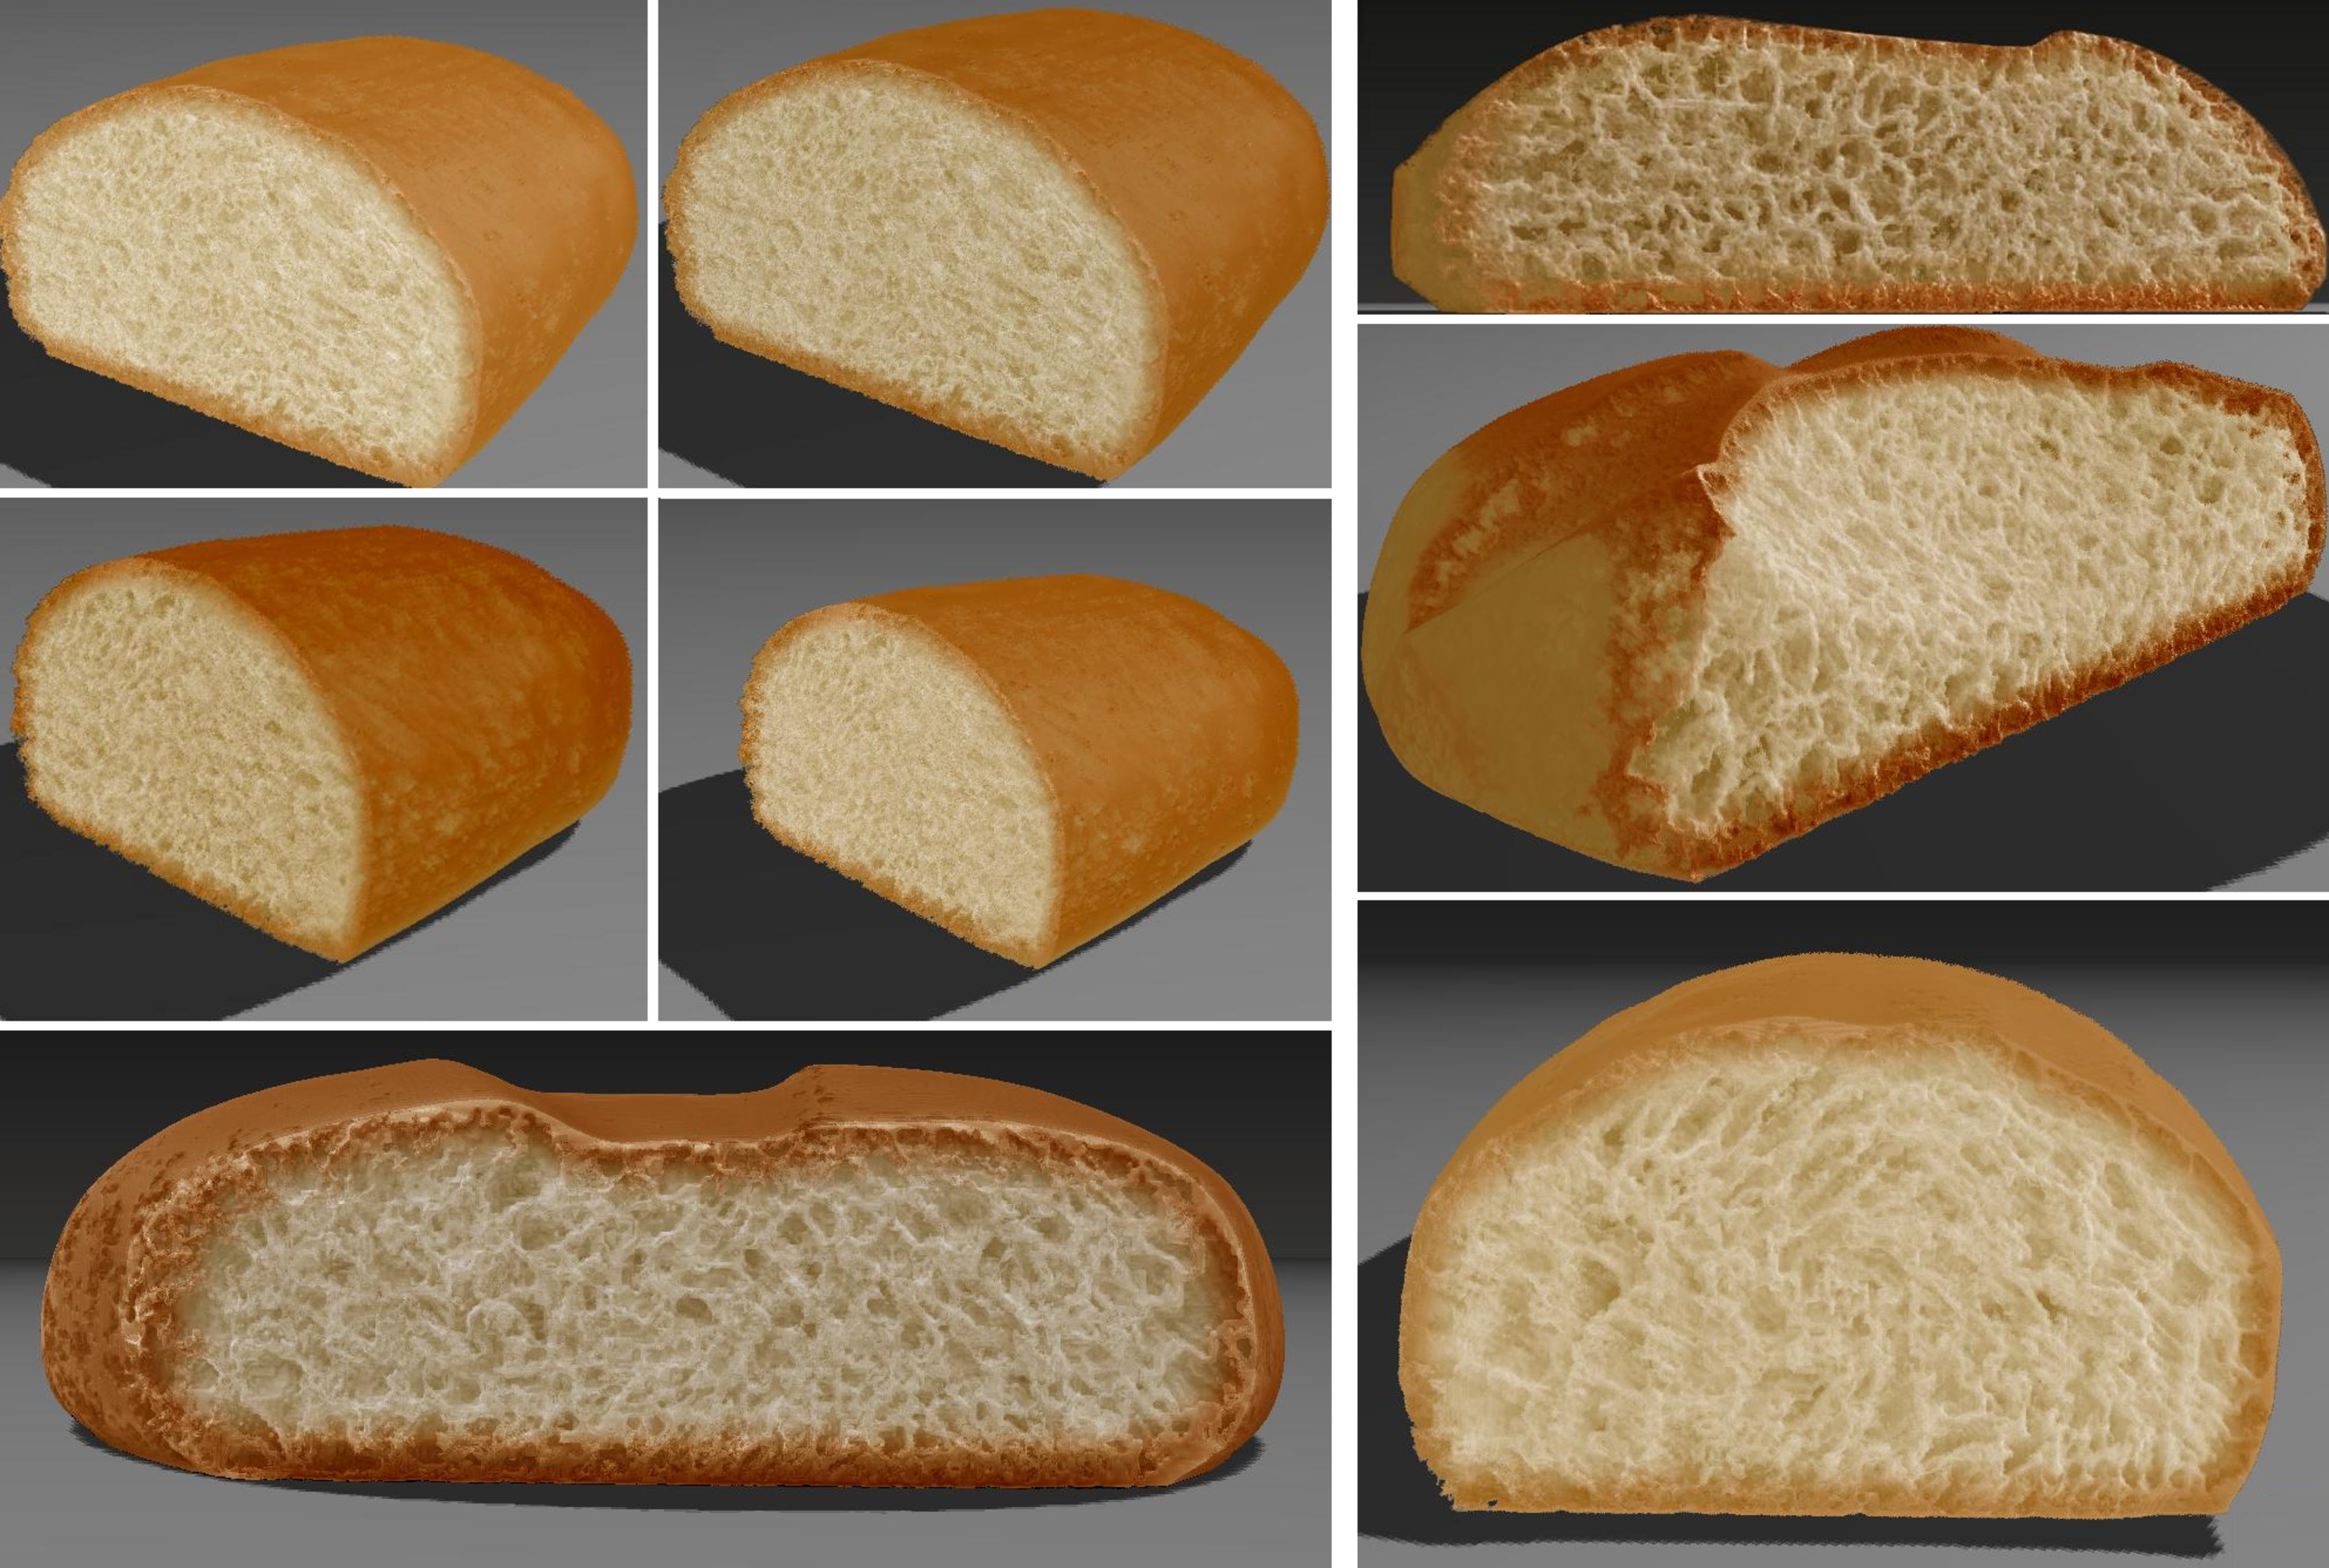
\includegraphics[width=12cm]{figures/Fig12CAVW}}
  \caption[Panes renderizados, utilizando diferentes geometrías y parámetros de renderizado]{Panes renderizados, utilizando diferentes geometrías y parámetros de renderizado. La imagen muestra que el método simula diferentes apariencias de panes.}
  \label{fg:Fig12}
\end{figure}


\subsection*{Tiempos de Cómputo}

Todas las imágenes fueron obtenidas en tasas de refresco de tiempo real (cuadros por segundo o \acrshort{FPS} mayor que $30$), ver Tabla \ref{tab:tiemposrenderizado}.
La eficiencia del proceso se resiente cuando el coeficiente de absorción resulta muy bajo, lo cual provoca que el material renderizado sea casi transparente, necesitándose evaluar más puntos en los rayos a recorrer antes de llegar al límite inferior de transmitancia.
Otro parámetro importante está dado por la cantidad de puntos a evaluar, ya que para cada paso computamos la transmitancia hacia la luz por medio de un rayo secundario.
Experimentalmente encontramos que utilizar $140$ o más pasos produce imágenes razonables para esponjas, pero se necesitan $300$ o más pasos para obtener imágenes razonables de panes, ver Fig.~\ref{fg:stepcount}.


\begin{figure}
  \centerline{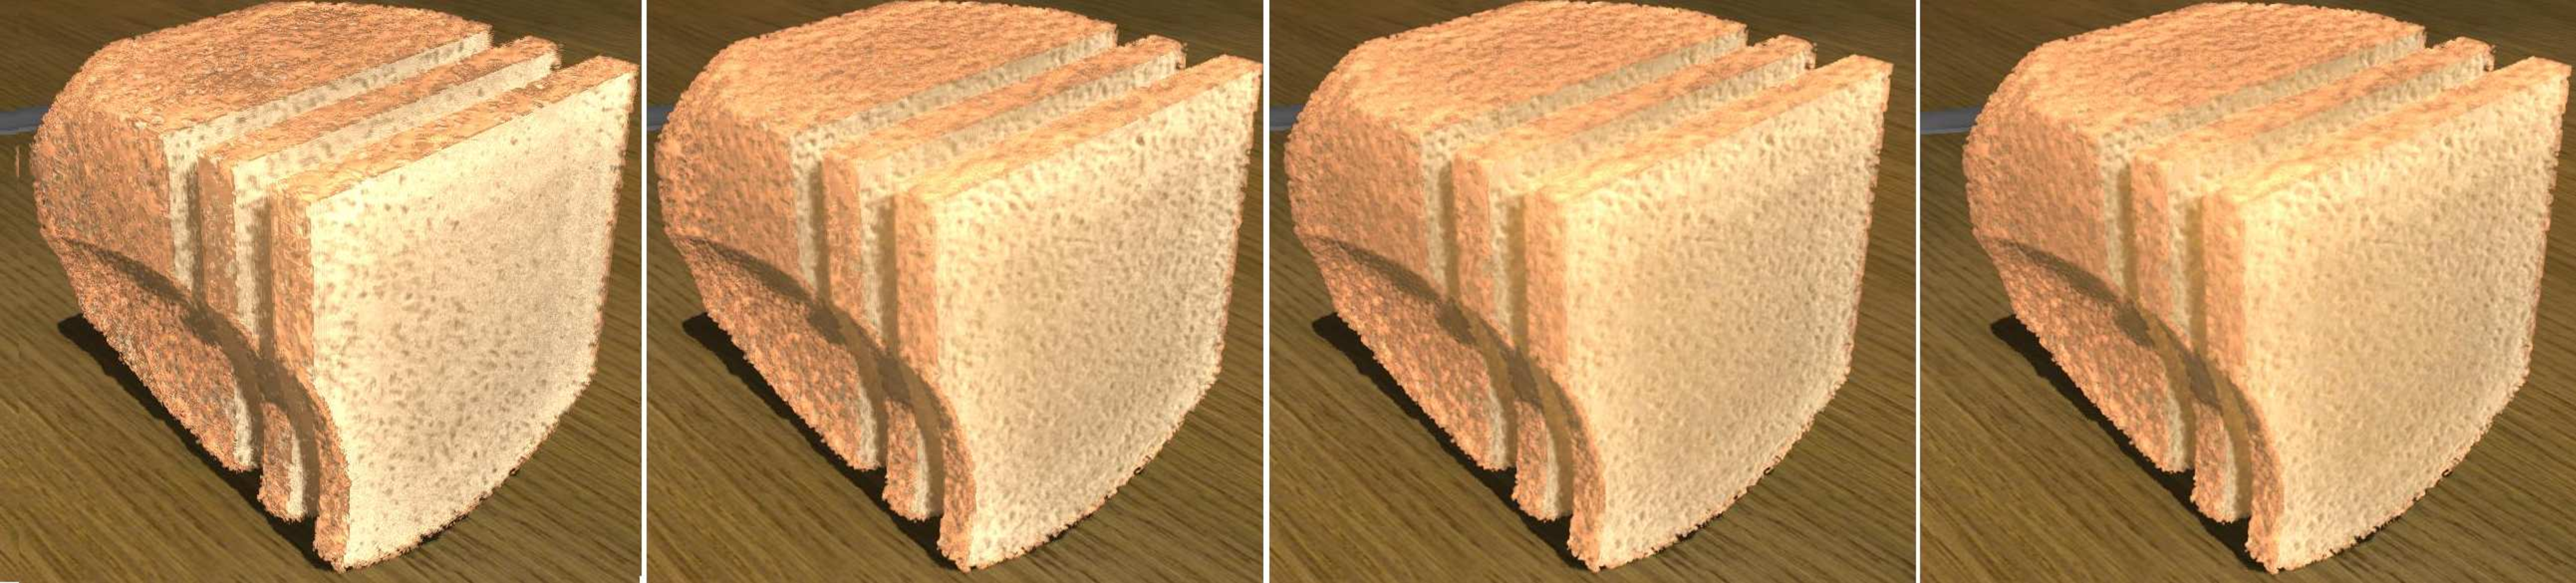
\includegraphics[width=12cm]{figures/stepcount}}
  \caption[Tiempos de cómputo de acuerdo a la cantidad de pasos utilizados]{Tiempos de cómputo de acuerdo a la cantidad de pasos utilizados. La imagen muestra que utilizar $300$ pasos del rayo produce imágenes razonables en tiempo real.}
  \label{fg:stepcount}
\end{figure}

La Tabla \ref{tab:rayossecundarios} muestra que los rayos secundarios constituyen el principal cuello de botella, lo cual resulta lógico, dado que a cada paso del rayo principal, el mismo computa un rayo secundario hacia la luz, mostrando tiempo cuadrático respecto a la cantidad de pasos.


\begin{table}[htb]
\centering
\begin{tabular}{|c|c|c|}
\hline &  Pan & Esponja \\
\hline
\hline
 FPS promedio & 42.6 & 57.4\\
\hline
 Puntos de evaluación &  440  & 187 \\
\hline
 Coeficiente de Absorción &  15  & 3.5 \\
\hline
\end{tabular}
\caption{Tiempos de renderizado y parámetros de las imágenes de prueba.}
\label{tab:tiemposrenderizado}
\end{table}

\begin{table}[htb]
\centering
\begin{tabular}{|c|c|c|c|c|c|c|}
\hline
 Pasos del rayo         & 128 &  256 \\
\hline
\hline
 Tiempo total shaders   & 10 ms &  32.5 ms \\
\hline
 Rayo Principal         & 2 ms  & 5 ms  \\
\hline
 Rayos Secundarios      &  8 ms & 27.5 ms  \\
\hline
\end{tabular}
\caption[Tiempos de renderizado en milisegundos]{Ejemplo típico de tiempos de renderizado en milisegundos. La tabla muestra que la mayor parte de los cómputos son debidos a los rayos secundarios.}
\label{tab:rayossecundarios}
\end{table}


En regiones con corteza, la velocidad del método resulta superior, ya que se puede obtener la apariencia deseada con un coeficiente de absorción mayor, es decir, los rayos necesitarán menos pasos para alcanzar el umbral inferior de transmitancia.

\subsection{Otros Materiales y Efectos}
Como fue mostrado en el capítulo anterior, es posible obtener imágenes que asemejan otros materiales (ver Fig.~\ref{fg:fig6}), variando parámetros técnicos y artísticos del modelo.
En las imágenes de prueba pueden distinguirse un budín (izquierda), un pedazo de torta (medio) y una esponja (derecha).
En el caso de la esponja se modificaron los parámetros que definen la función de densidad, utilizando una mayor aleatoriedad, para producir una textura más homogénea.

En las Figs.~\ref{fg:sponges} y \ref{fg:Fig14} se muestran esponjas y piedras porosas sintetizadas con el mismo procedimiento, utilizando distintos valores para la aleatoriedad, cantidad de burbujas iniciales, la especularidad, y el coeficiente de absorción.
La retro-iluminación también se aproxima en este modelo (ver Fig. \ref{fg:fig7}).
En esa imagen puede apreciarse una esponja retro-iluminada junto con la propagación de luz a través del volumen que representa.
Este efecto surge como una consecuencia natural del algoritmo volumétrico basado en RTE utilizado en este capítulo.

\begin{figure*}[htb!]
  \centerline{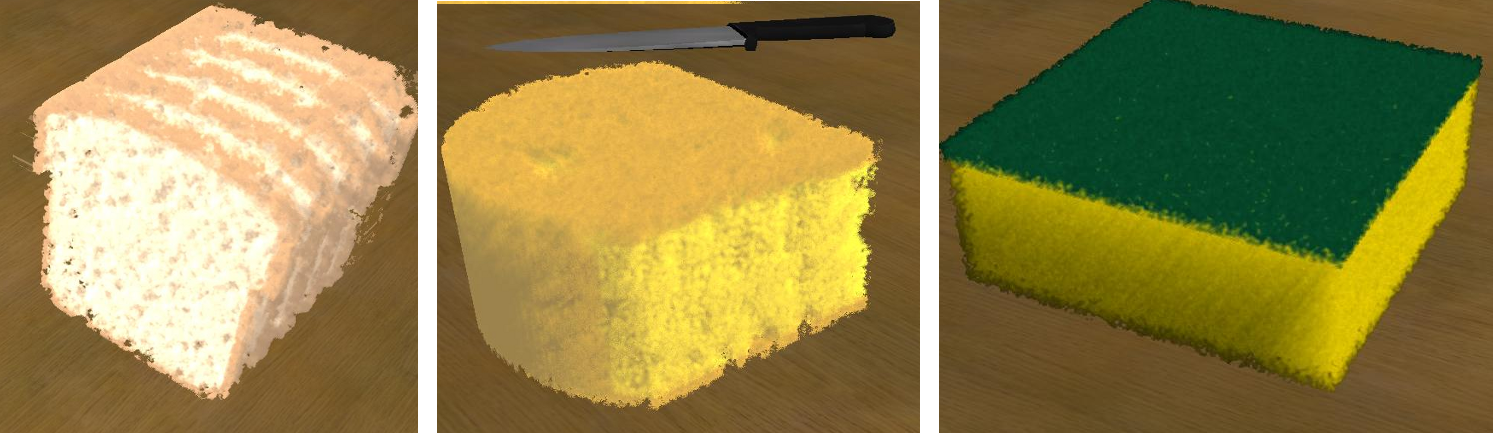
\includegraphics[width=12cm]{figures/fig6}}
  \caption[Budín, torta y esponja renderizados]{Distintos materiales obtenidos a partir de diferentes configuraciones de parámetros. De izquierda a derecha: budín, torta y esponja. }
  \label{fg:fig6}

\end{figure*}

\begin{figure*}[htb!]
  \centerline{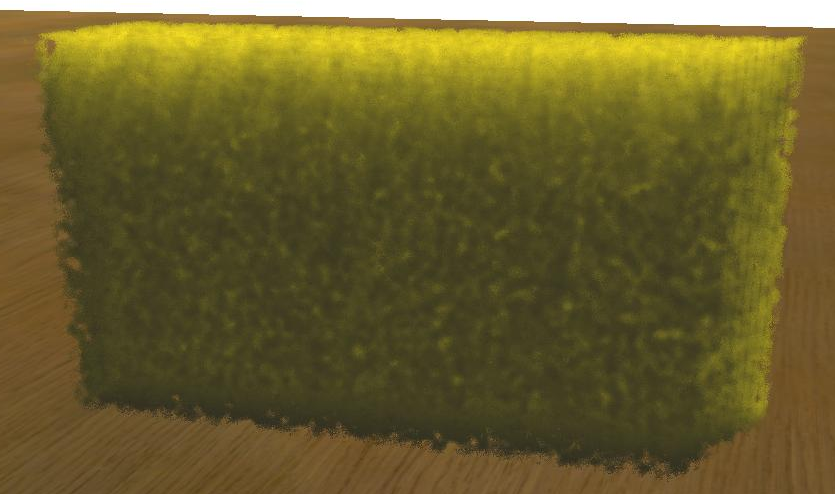
\includegraphics[width=5cm]{figures/fig7}}
  \caption[Esponja retro-iluminada.]{Esponja renderizada en tiempo real mostrando retro-iluminación. La misma resulta consecuencia directa de la utilización de un modelo volumétrico de propagación de la energía radiante, sobre medios semi-transparentes.}
  \label{fg:fig7}
\end{figure*}


\begin{figure}
  \centerline{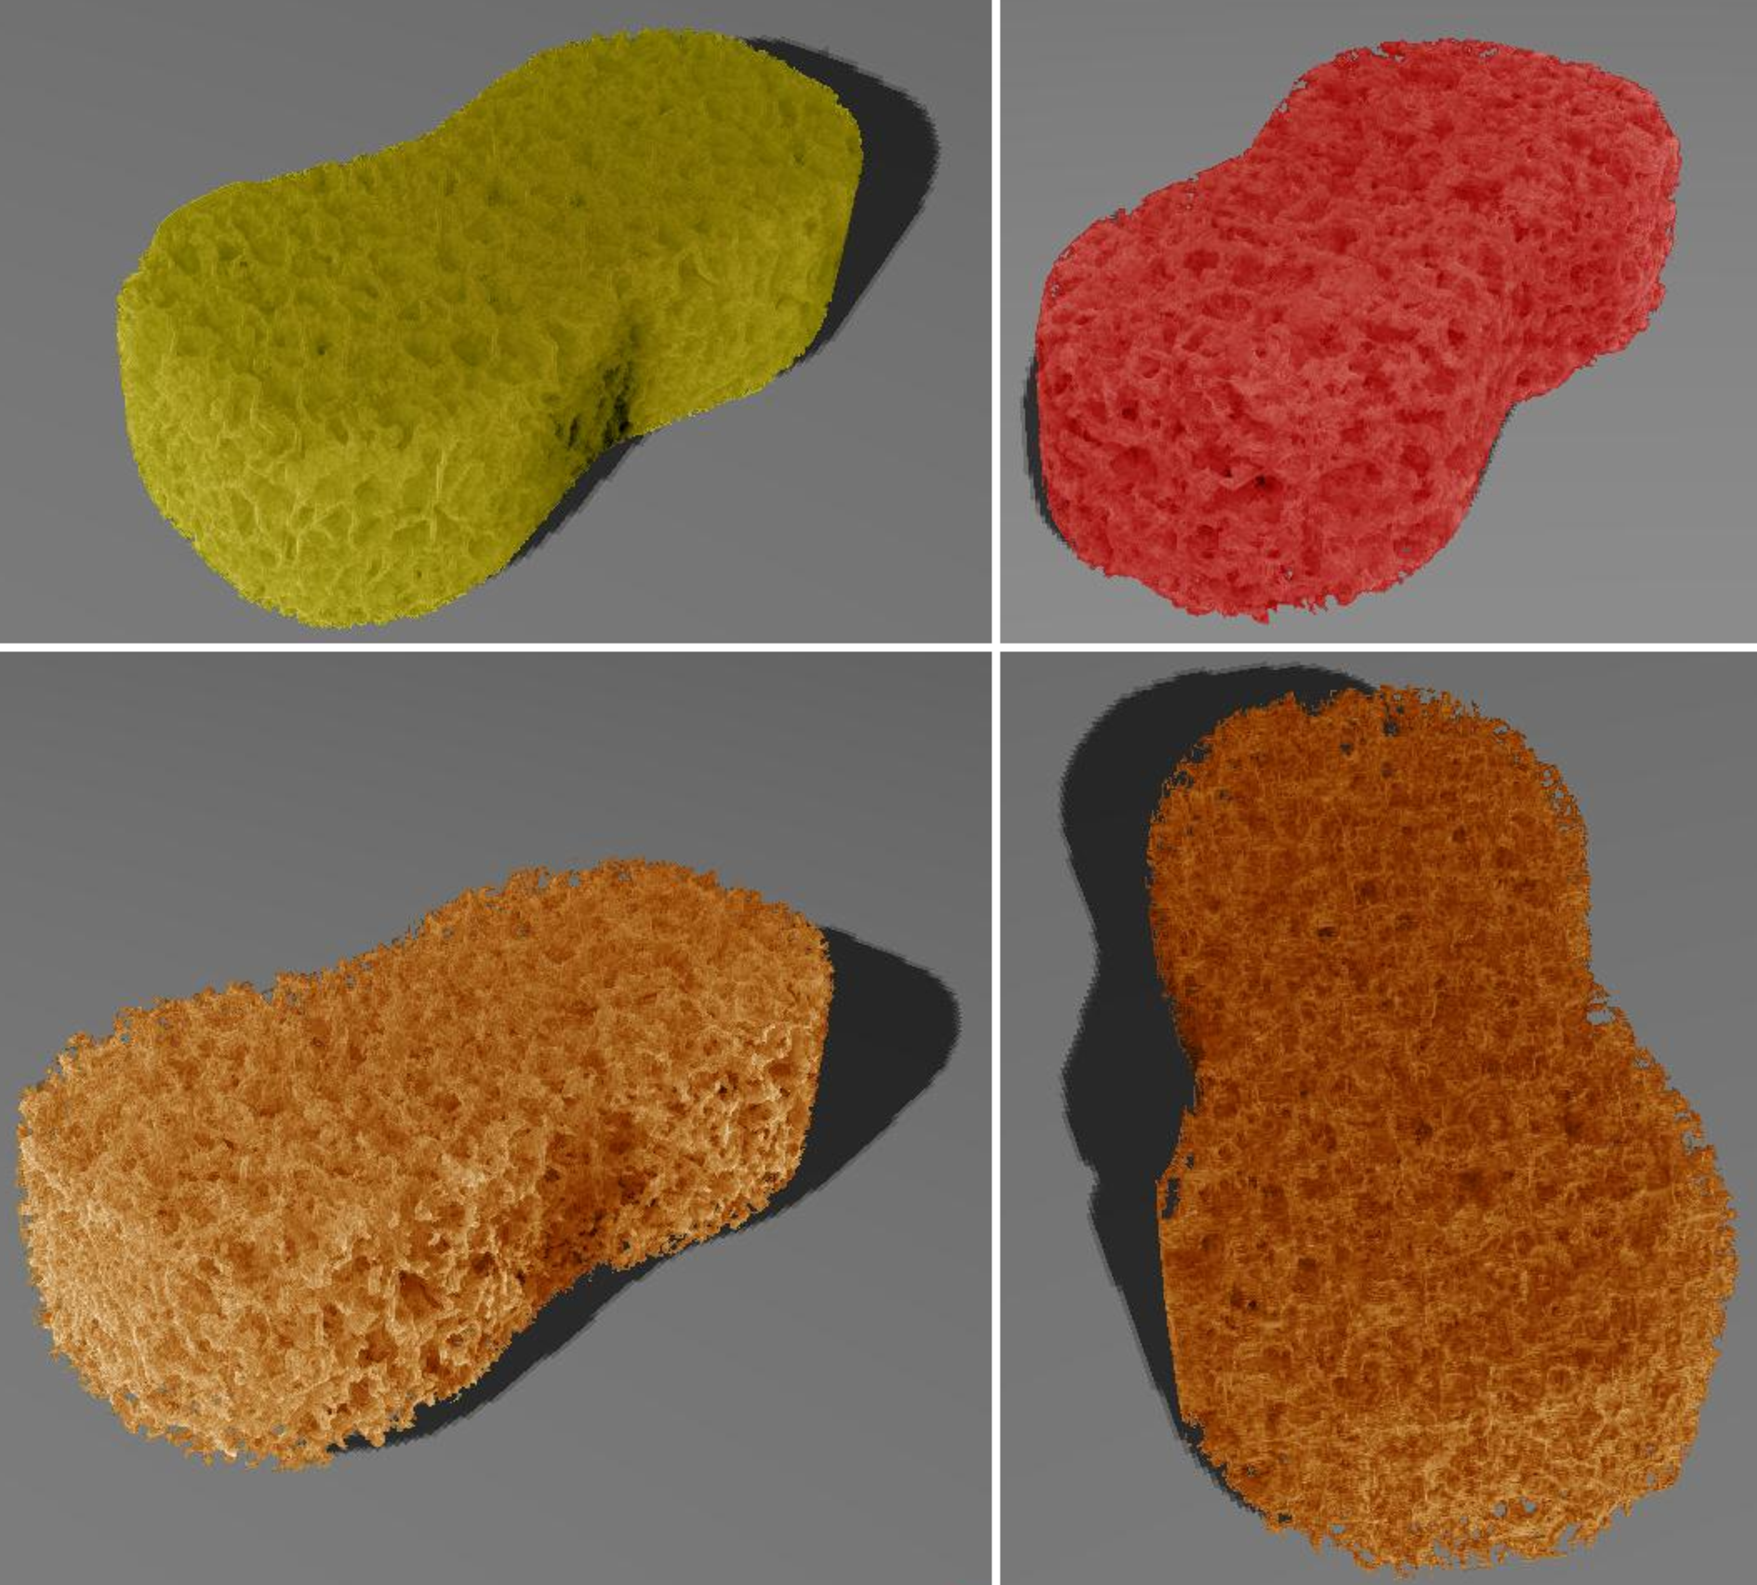
\includegraphics[width=9cm]{figures/Fig13CAVW}}
  \caption[Esponjas renderizadas]{Esponjas renderizadas. La textura volumétrica que representa la geometría fue generada con un valor de {\em aleatoriedad} mayor que en el caso del pan. La geometría resultante posee tamaños y orientaciones de burbujas homogéneos.}
  \label{fg:sponges}
\end{figure}

\begin{figure}
  \centerline{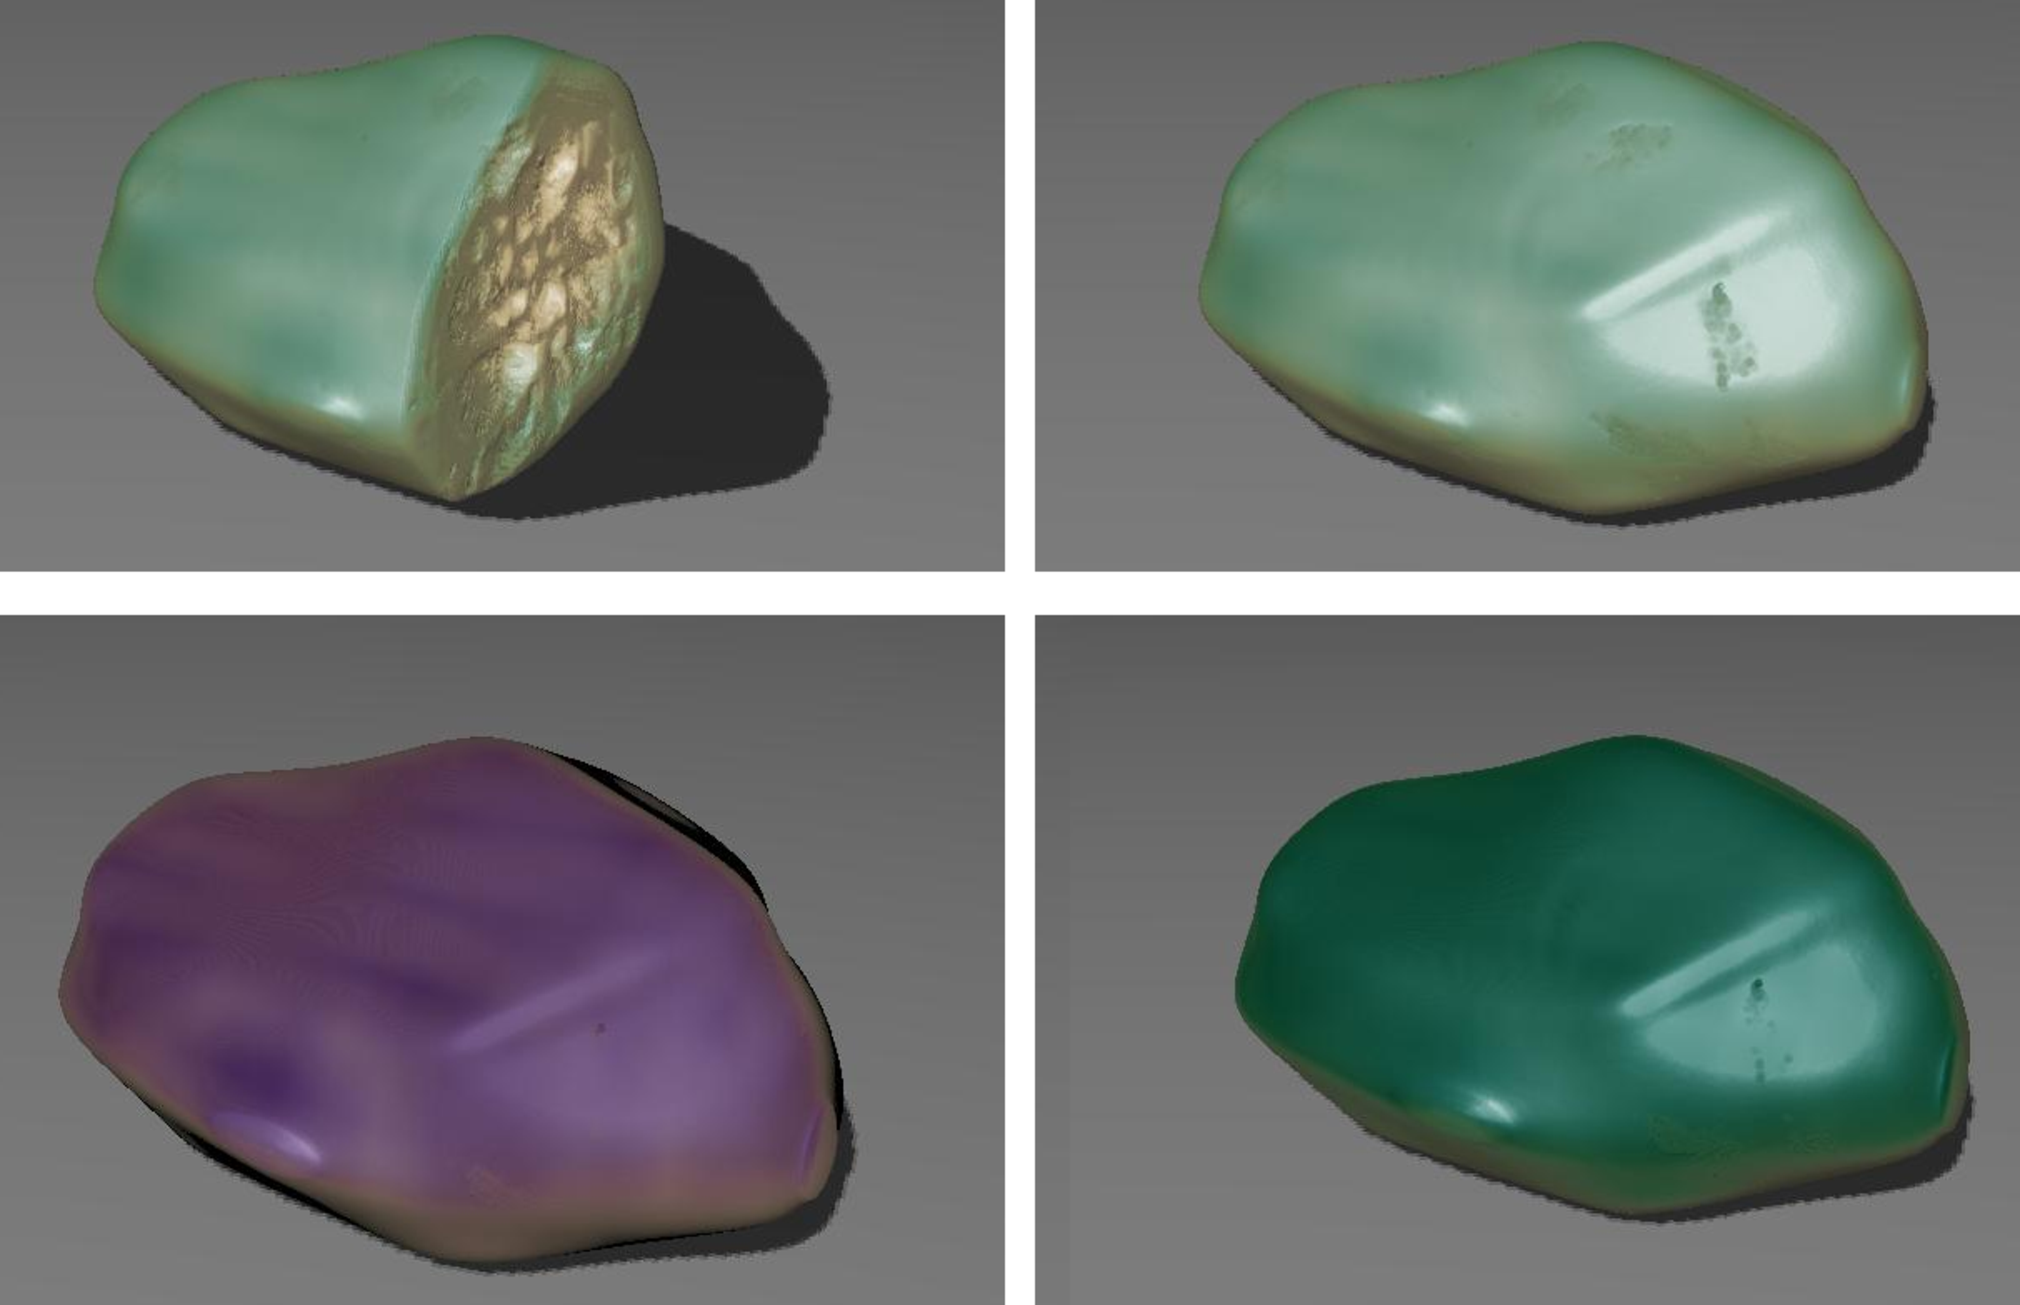
\includegraphics[width=12cm]{figures/Fig14CAVW}}
  \caption[Piedras renderizadas]{Piedras renderizadas. Se utilizó un menor número de partículas en la generación de este material. El índice de absorción fue incrementado en el renderizado para prevenir una difusión lumínica excesiva.}
  \label{fg:Fig14}
\end{figure}

\subsection{Renderizado Multi-escala}
Debido a limitaciones del hardware, el tamaño de la textura influencia el rendimiento final del algoritmo.
Una textura de resoluciones mayores a $256^{3}$ voxels compromete el desempeño de tiempo real del algoritmo de renderizado.
Sin embargo, como fue demostrado, para aumentar la calidad gráfica de la imagen es necesario superar esta barrera.

Una posible solución a este conflicto está constituida por la utilización de más de una textura volumétrica en el modelado, donde una de ellas modela las características de mayor tamaño del objeto (por ejemplo, sus burbujas más grandes), y la otra se utiliza para representar detalles de menor escala.
El resultado de la utilización de más de una textura puede observarse en la Fig.~\ref{fg:multiscale}, donde la diferencia es claramente visible.
La segunda textura produce la ilusión de un objeto con una estructura mucho más rica.
La implementación de esta técnica simplemente reemplaza el valor de la textura, representando los detalles de mayor escala, en el voxel siendo muestreado, con la combinación de los valores de ambas texturas en ese voxel, donde la textura que representa los detalles de menor escala se muestrea a mayor frecuencia.
Es decir, si la posición del voxel es $(x,y,z)$, la primera textura se muestrea en esa posición, y la segunda textura se muestrea en $N\times (x, y,z)$, con $N \in \mathbb{R}$.
A medida que $N$ crece, se representan detalles de menor escala en la textura final (por ejemplo, burbujas más chicas).
Estos valores pueden multiplicarse o sumarse para producir el valor final del voxel antes de ser renderizado.

El costo computacional agregado está representado por muestrear dos texturas en lugar de una.
Si bien el muestreo es una operación costosa, el tiempo total resulta mucho menor al costo computacional de trabajar con texturas de mayores dimensiones.
La textura que se muestrea a distintas escalas debe poseer cierta coherencia en sus bordes (arriba/abajo, izquierda/derecha, etc.), para poder ser ensamblada sin que se note el efecto del muestreo.

\begin{figure}
  \centerline{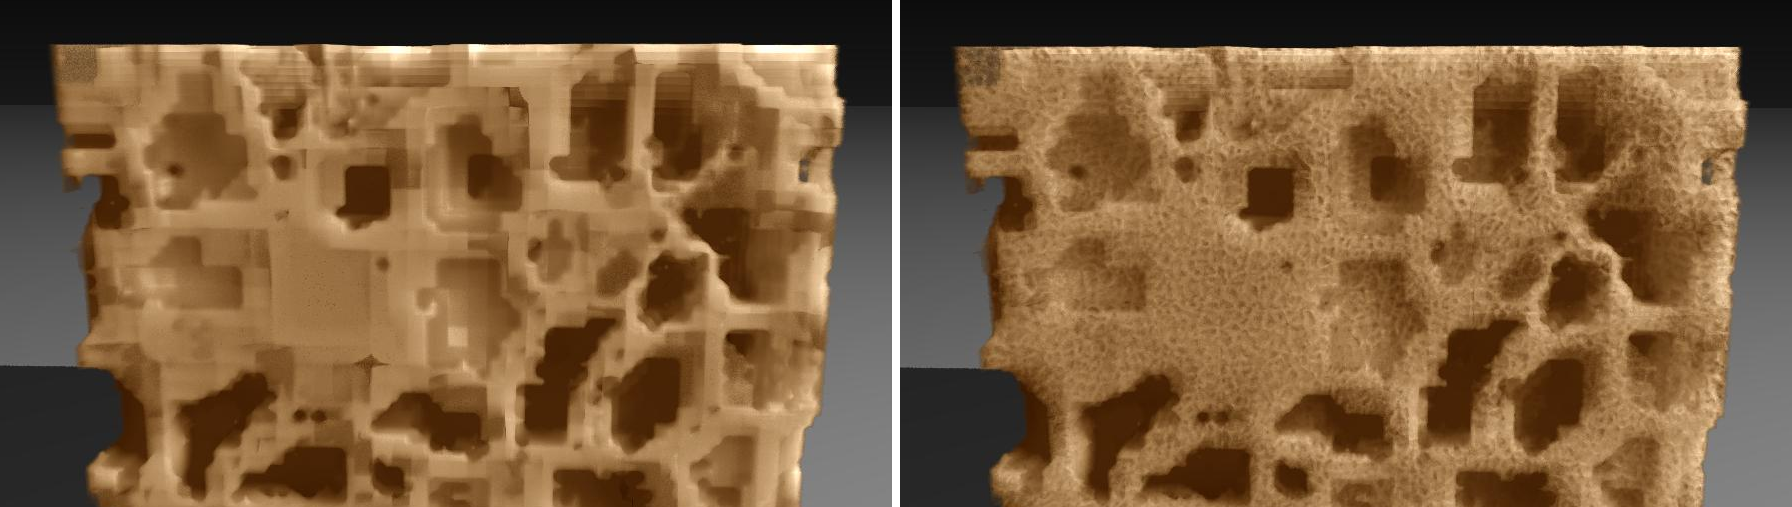
\includegraphics[width=12cm]{figures/multiscale}}
  \caption[Estructura porosa utilizando una y dos escala de muestreo]{Estructura porosa utilizando una única escala de muestreo (izquierda) y dos (derecha). Se puede apreciar claramente el aumento en el nivel de detalle resultante en la imagen, a un costo computacional aceptable.}
  \label{fg:multiscale}
\end{figure}

\section{Discusión}

Hasta donde podemos observar en la literatura, en el renderizado de panes y otros materiales porosos, este constituye el primer trabajo que involucra tasas de refresco de tiempo real, sin la utilización de estructuras intermedias, procesos de captura onerosos, o post-procesamientos.
La literatura previa incluye pocos trabajos, como por ejemplo \cite{Cho2007}, pero las comparaciones con este método no son posibles, ya que los detalles claves del desarrollo no fueron explicados (tiempos de cómputo, método de renderización).
El método propuesto resulta compatible con el renderizado de ráster en tiempo real disponible en las GPUs actuales, contando con la capacidad de producir un material realista.
El método puede ser integrado con facilidad en cualquier motor $3D$ basado en shaders.
Además, la técnica de mapeo de sombras permite integrar el material en escenas de una manera natural.

%3) Recordamos que las imagenes obtenidas fueron buenas, y que obtuvimos otros materiales cambiando pocos parametros

El algoritmo de renderizado resulta lo suficientemente flexible, modelando diferentes materiales, como pan, esponjas, y tortas, modificando unos pocos parámetros.
Otros materiales porosos como pizzas, quesos, y otros, pueden ser fácilmente obtenidos definiendo geometrías adecuadas y parámetros de transmitancia y cantidad de pasos.
Es decir, se pueden obtener diversos materiales con el mismo método.
Además, nuestra representación volumétrica permite realizar cortes en tiempo real en la miga y corteza del pan.
Esto puede resultar de gran ayuda en diversas aplicaciones, entre las cuales encontramos video juegos.

Respecto al modelo de iluminación, el éxito visual obtenido por el método a la hora de obtener una apariencia que semeja al pan en tiempo real, parece estar dado por la utilización de oclusión ambiente, además de los agregados discutidos sobre el algoritmo básico de DVR.
El término de oclusión de ambiente proporcionó una textura mucho más detallada, mostrando una mayor complejidad y riqueza subyacente.
Otros efectos introducidos, como el reflejo especular de Phong, también incidieron sobre el realismo final.
Sin embargo, métodos especulares más sofisticados (por ejemplo, Cook-Torrance \cite{Cook1982}) no aportaron mayores detalles sobre la apariencia las imágenes.

%5)Tiempos de cómputo

Los tiempos de cómputo alcanzados fueron adecuados para obtener tasas de refresco de tiempo real en computadoras estándares al año de publicación de la presente tesis (utilizamos una placa de video nVidia GTX 480, junto con una \acrshort{CPU} Intel(R) i5).
En la gran mayoría de los casos, las tasas de refresco alcanzadas fueron de tiempo real.
Los únicos casos que no lograron dichos tiempos ocurrieron cuando el objeto a ser renderizado ocupó una porción bastante considerable de la pantalla, ya que el método está implementado en el shader de fragmentos.
Los tiempos de cómputo finales dependen de la cantidad de pasos utilizados, el coeficiente de absorción y el umbral inferior de transmitancia.

Adicionalmente, diferentes materiales cuentan con diferentes tiempos de cómputo para su renderización.
Por ejemplo, un tiempo de cómputo adecuado para simular esponjas resulta más bajo que aquél que se necesita para modelar migas de panes.
Esto se debe al hecho de que el método necesita más pasos para capturar las burbujas macroscópicas del pan.

Las GPUs actuales poseen límites en las dimensiones de las texturas volumétricas que pueden soportar.
Esto limita la calidad de las imágenes que podemos obtener, ya que a mayor resolución, fue demostrado que puede obtenerse un mayor detalle y realismo en las imágenes.
Por lo tanto, las aplicaciones en tiempo real deben limitar la resolución de la textura que se carga en la GPU.
En otras palabras, acercamientos extremos a la estructura a ser renderizada puede dar lugar áreas homogéneas (sin detalle).
Esta limitación está relacionada al tamaño de textura de la GPU, y será eventualmente superado con la mejora del hardware de la próxima generación de GPUs.
En aplicaciones donde el tiempo de cómputo constituye un factor crucial, se permite la utilización de texturas lo suficientemente grandes para dar lugar a imágenes foto-realísticas.
La utilización de un modelo multiescala, como fue discutido, puede subsanar estas deficiencias.

\section{Conclusiones}

En este capítulo hemos aplicado el modelo de transmitancia del renderizado directo de volúmenes, utilizando la GPU, sobre un campo escalar tridimensional representando la estructura de la miga del pan (la cual fue computada en el capítulo anterior).
Se obtuvieron imágenes realistas en tiempo real.
Por medio de la utilización de texturas de mayores dimensiones se obtuvieron imágenes con mayor detalle, pero a tasas de refresco menores.
Si bien el algoritmo de renderizado no es novedoso, sí lo es su aplicación en los materiales porosos discutidos, y la obtención de tasas de tiempo real a partir del mismo.

El algoritmo presentado fue implementado en el shader de fragmentos utilizando componentes especulares y difusas, cómputo de normales y oclusión de ambiente.
Los resultados alcanzados son comparables al estado del arte, obteniendo imágenes que simulan el material en tiempo real con gran realismo.
El método presenta aplicaciones en diversas áreas, como video juegos, juegos serios \cite{Susi2007} y renderizado foto-realista.
Estas técnicas son mucho más simples y no presentan las desventajas de otros métodos, como procesos de captura, generación de mallas o post-procesos.
Las mismas fueron presentadas en un congreso y revista nacionales \cite{Baravalle2014}, y están en revisión en una revista internacional.
Estos resultados demuestran que la elección de una representación volumétrica resulta adecuada para estos materiales porosos.



